\section{LÝ THUYẾT}
\subsection{Vi xử lý Atmega328P}
ATmega328P là vi điều khiển 8-bit CMOS công suất thấp dựa trên kiến trúc AVR RISC nâng cao. Đây là dòng vi điều khiển phổ biến (thường thấy trong Arduino Uno), được lựa chọn nhờ sự cân bằng giữa hiệu năng xử lý và khả năng tiết kiệm năng lượng. Với khả năng thực thi các lệnh mạnh mẽ trong một chu kỳ xung nhịp đơn, ATmega328P đạt thông lượng xấp xỉ 1 MIPS trên mỗi MHz, cho phép tối ưu hóa mức tiêu thụ năng lượng so với tốc độ xử lý. Chip hỗ trợ đầy đủ các chuẩn giao tiếp phổ biến như UART, SPI, I2C và tích hợp sẵn ADC độ phân giải cao, phù hợp cho các ứng dụng điều khiển và thu thập dữ liệu.
\begin{figure}[h!]
    \centering
    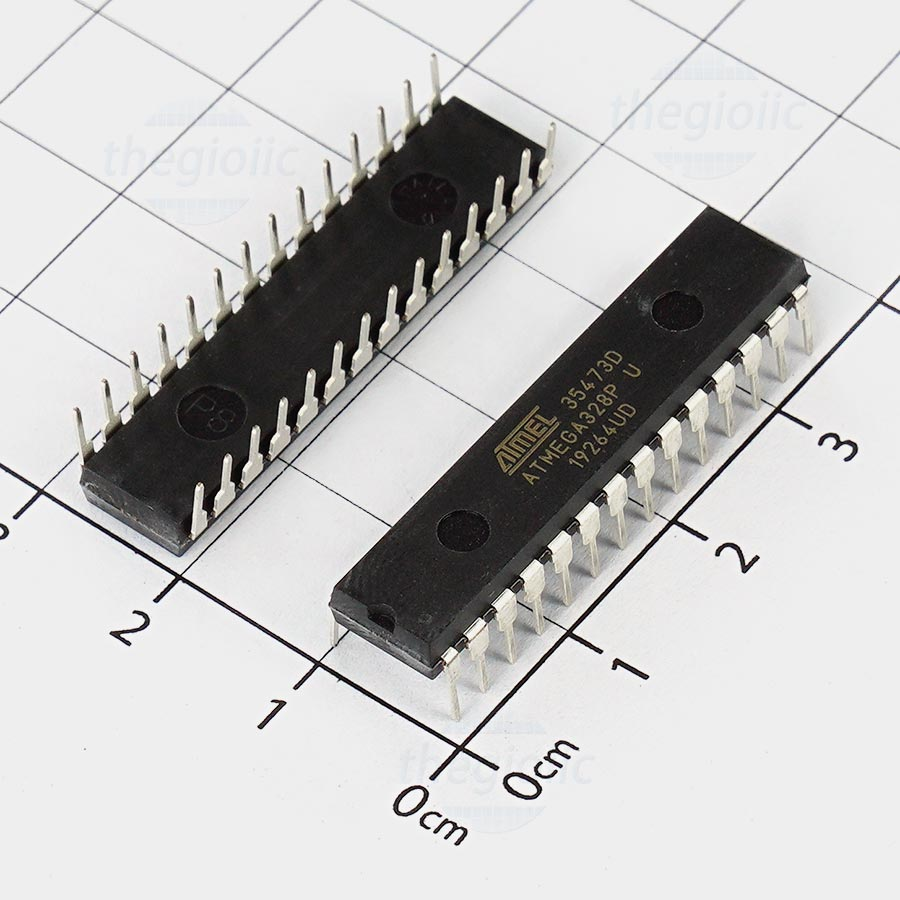
\includegraphics[width = 0.3\textwidth]{img/1.png}
    \caption{Vi xử lý ATmega328P}
\end{figure}\\
\textbf{Thông số linh kiện:}
\begin{itemize}
    \item MCU: ATmega328P (8-bit AVR RISC).
    \item Điện áp hoạt động: 1.8V - 5.5V (Thường dùng ổn định ở 2.7V - 5.5V).
    \item Tần số hoạt động: Tối đa 20 MHz.
    \item Hiệu năng: Lên đến 20 MIPS tại 20 MHz.
    \item Bộ nhớ Flash (Lưu chương trình): 32 KB (Có khả năng nạp lại ngay trên mạch - ISP).
    \item Bộ nhớ SRAM (Lưu dữ liệu tạm): 2 KB.
    \item Bộ nhớ EEPROM (Lưu dữ liệu bền vững): 1 KB.
    \item Số chân I/O: 23 chân lập trình được (trên gói DIP-28).
    \item Bộ định thời (Timer/Counter):
        \begin{itemize}
            \item 2 bộ Timer/Counter 8-bit (Timer0, Timer2).
            \item 1 bộ Timer/Counter 16-bit (Timer1).
        \end{itemize}
    \item Kênh PWM: 6 kênh (Dùng điều khiển động cơ, độ sáng LED,...).
    \item Bộ chuyển đổi ADC: Độ phân giải 10-bit, 6 kênh (hoặc 8 kênh trên gói TQFP/MLF).
    \item Giao tiếp ngoại vi:
        \begin{itemize}
            \item 1 bộ USART (Truyền thông nối tiếp).
            \item 1 bộ SPI (Serial Peripheral Interface).
            \item 1 bộ TWI (Tương thích chuẩn I2C, 2 dây).
        \end{itemize}
    \item Các tính năng khác: Watchdog Timer, ngắt ngoài, cảm biến nhiệt độ tích hợp.
    \item Nhiệt độ hoạt động: -40°C đến +85°C.
\end{itemize}
\subsection{LCD 1602}
Trong phân khúc các thiết bị hiển thị giá rẻ nhưng vẫn đảm bảo khả năng hiển thị thông tin trực quan (như thời gian, trạng thái cảm biến), nhóm lựa chọn LCD 1602. Đây là loại màn hình ký tự (Character LCD) sử dụng IC điều khiển HD44780 rất phổ biến, hỗ trợ hiển thị 16 ký tự trên 2 dòng. LCD 1602 có ưu điểm là giao tiếp đơn giản với vi điều khiển (như ATmega328P) thông qua chuẩn 4-bit hoặc 8-bit, độ bền cao và tiêu thụ ít năng lượng.
\begin{figure}[h!]
    \centering
    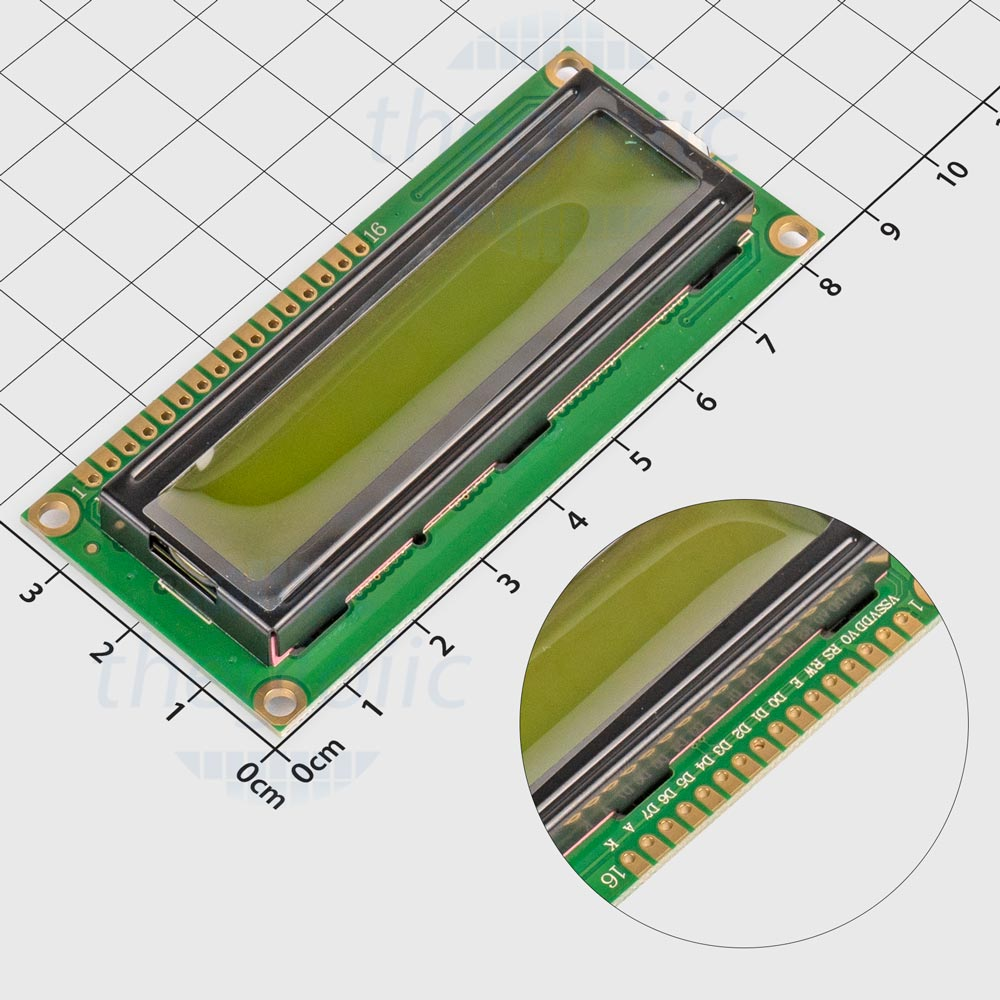
\includegraphics[width = 0.35\textwidth]{img/2.png}
    \caption{LCD 1602}
\end{figure}

\noindent\textbf{Thông số kỹ thuật:}
\begin{itemize}
    \item Điện áp hoạt động (VCC): 5V DC (Thường hoạt động ổn định trong khoảng 4.7V - 5.3V).
    \item Dòng điện tiêu thụ: Khoảng 1mA (không đèn nền) và lên đến 20-30mA (có đèn nền).
    \item IC điều khiển (Controller): HD44780 hoặc tương đương.
    \item Khả năng hiển thị: 16 cột x 2 hàng (tối đa 32 ký tự).
    \item Kích thước điểm ảnh: 5x8 điểm (dot matrix) cho mỗi ký tự.
    \item Màu sắc: Thường là chữ trắng nền xanh dương hoặc chữ đen nền vàng xanh.
    \item Giao tiếp: Song song (Parallel) 4-bit hoặc 8-bit.
\end{itemize}
\textbf{Chức năng các chân cơ bản:}
\begin{itemize}
    \item Chân 1 (VSS) $\&$ Chân 2 (VDD): Cấp nguồn GND và +5V cho màn hình.
    \item Chân 3 (V0/VEE): Điều chỉnh độ tương phản (Contrast) của màn hình (thường nối với biến trở).
    \item Chân 4 (RS - Register Select): Lựa chọn thanh ghi. Mức thấp (0) để gửi lệnh điều khiển, mức cao (1) để gửi dữ liệu hiển thị.
    \item Chân 5 (RW - Read/Write): Chọn chế độ Đọc hoặc Ghi. Thường nối đất (GND) để chọn chế độ Ghi dữ liệu.
    \item Chân 6 (E - Enable): Chân cho phép (xung kích hoạt để LCD nhận dữ liệu).
    \item Chân 7-14 (D0 - D7): 8 chân dữ liệu (Data bus). Trong chế độ 4-bit chỉ sử dụng D4-D7.
    \item Chân 15 (A) $\&$ Chân 16 (K): Nguồn cho đèn nền (Anode nối 5V, Cathode nối GND).
\end{itemize}
\subsection{Module LED MATRIX 8x8 VÀ IC MAX7219}
Để hiển thị các ký tự, hình ảnh đơn giản hoặc các hiệu ứng ánh sáng mà vẫn tiết kiệm tài nguyên vi điều khiển, nhóm quyết định sử dụng Module LED Matrix 8x8 tích hợp IC điều khiển MAX7219.

Việc điều khiển trực tiếp một ma trận LED 8x8 thông thường đòi hỏi tới 16 chân GPIO và vi xử lý phải liên tục thực hiện quét LED (multiplexing) để duy trì hình ảnh. IC MAX7219 giải quyết vấn đề này bằng cách đảm nhận toàn bộ việc quét hiển thị, điều chỉnh độ sáng và chỉ yêu cầu giao tiếp qua 3 dây tín hiệu (Giao thức tương thích SPI). Ngoài ra, khả năng mắc nối tiếp (cascade) nhiều module lại với nhau giúp mở rộng diện tích hiển thị dễ dàng.
\begin{figure}[h!]
    \centering
    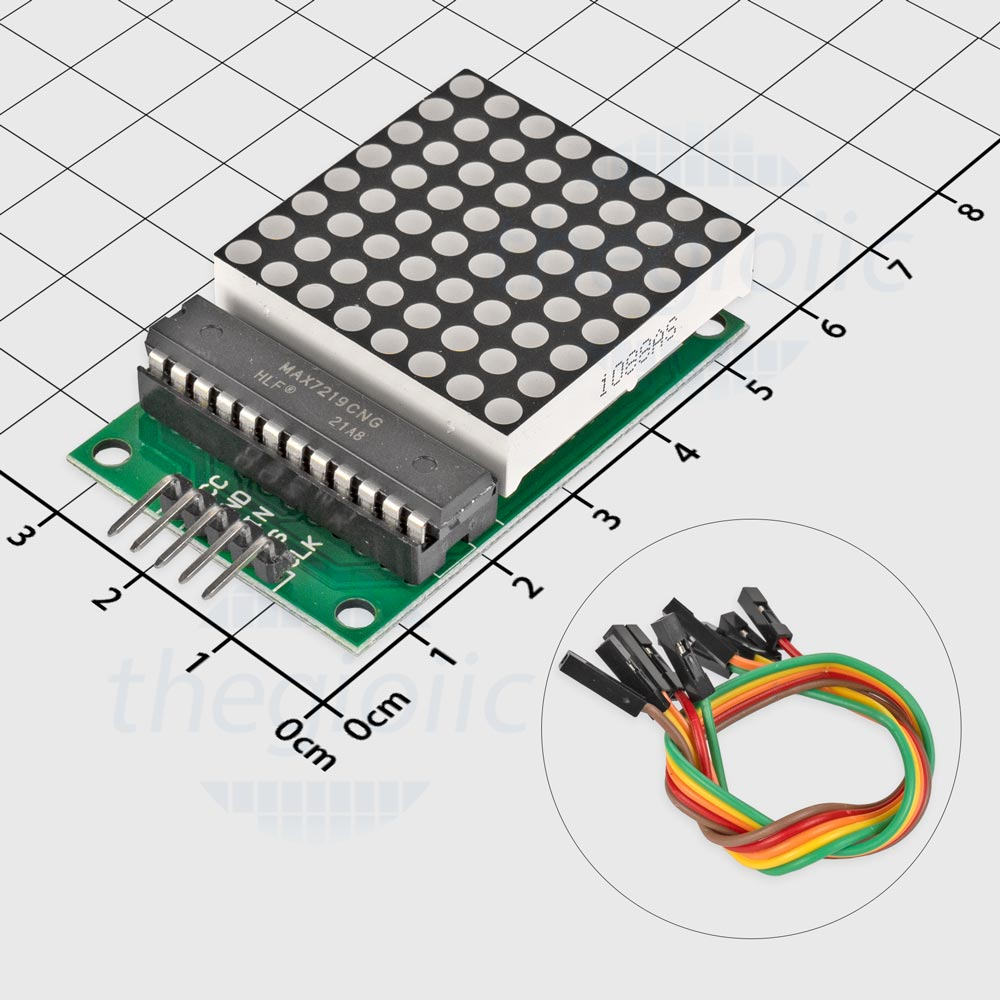
\includegraphics[width = 0.4\textwidth]{img/5.png}
    \caption{MAX7219 led matrix}
\end{figure}

\noindent\textbf{Thông số kỹ thuật:}
\begin{itemize}
    \item IC điều khiển: MAX7219 (Driver hiển thị LED Cathode chung, đầu vào/ra nối tiếp).
    \item Màu sắc hiển thị: Đỏ (phổ biến nhất), Xanh lá, hoặc Xanh dương.
    \item Điện áp hoạt động: 4.0V - 5.5V DC (Khuyến nghị 5V).
    \item Giao tiếp: Serial Interface (Tương thích SPI) gồm 3 dây: DIN, CS (LOAD), CLK.
    \item Tần số xung nhịp tối đa: 10 MHz.
    \item Khả năng điều khiển: 1 IC MAX7219 điều khiển được 64 LED đơn (hoặc 1 ma trận 8x8, hoặc 8 LED 7 thanh).
    \item Điều chỉnh độ sáng: Kỹ thuật số (16 mức độ sáng thông qua thanh ghi nội).
    \item Dòng điện tiêu thụ: Tối đa khoảng 330mA (khi bật tất cả LED độ sáng cao nhất).
\end{itemize}
\textbf{Chức năng các chân (Trên Module):}
\begin{itemize}
    \item VCC: Chân cấp nguồn dương (5V).
    \item GND: Chân cấp nguồn âm (0V).
    \item DIN (Data In): Chân nhận dữ liệu nối tiếp từ vi điều khiển.
    \item CS/LOAD (Chip Select): Chân chọn chip/chốt dữ liệu. Dữ liệu được chốt vào thanh ghi khi có sườn lên.
    \item CLK (Clock): Chân xung nhịp đồng bộ dữ liệu.
    \item DOUT (Data Out): Chân xuất dữ liệu sang module tiếp theo (dùng khi mắc nối tiếp nhiều LED Matrix).
\end{itemize}
\subsection{Mạch sạc pin TP4056}
Để giải quyết bài toán năng lượng cho thiết bị di động sử dụng pin Li-Ion/Li-Po đơn cell (3.7V), nhóm lựa chọn IC quản lý sạc TP4056. Đây là dòng chip sạc tuyến tính (linear charger) trọn gói, hoạt động theo cơ chế Dòng không đổi / Điện áp không đổi (CC/CV). Ưu điểm nổi bật của TP4056 là thiết kế đơn giản, giá thành thấp và không cần linh kiện cảm biến dòng hay diode chặn ngoài nhờ tích hợp kiến trúc PMOSFET bên trong, rất lý tưởng cho các ứng dụng sạc qua cổng USB.
\begin{figure}[h!]
    \centering
    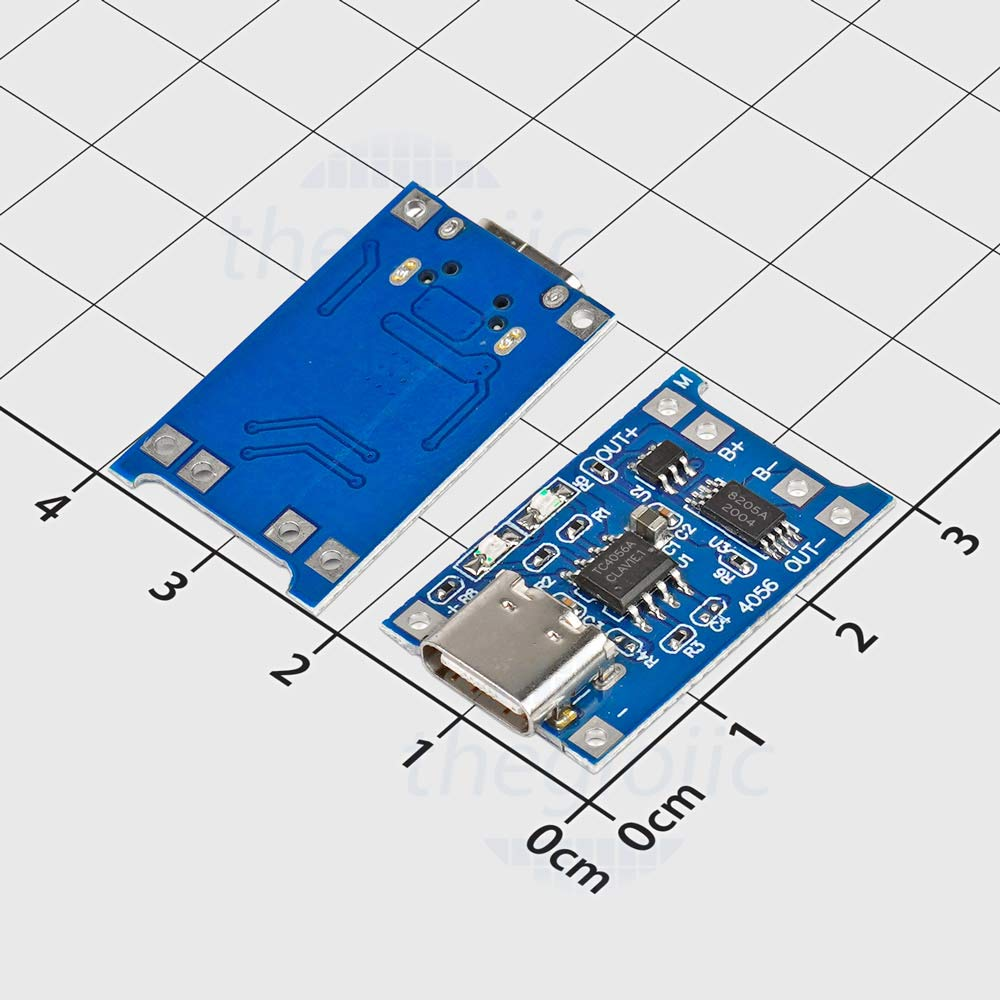
\includegraphics[width = 0.4\textwidth]{img/3.png}
    \caption{Mạch TP4056}
\end{figure}
\newpage
\noindent\textbf{Thông số kỹ thuật:}
\begin{itemize}
    \item Điện áp sạc: Cố định chính xác ở mức 4.2V.
    \item Dòng sạc tối đa: Có thể lập trình lên tới 1000mA (1A) chỉ qua một điện trở ngoài.
    \item Chu trình sạc: Tự động 3 giai đoạn: Sạc nhỏ giọt (khi pin < 2.9V), Sạc dòng không đổi (CC), Sạc áp không đổi (CV).
    \item Ngưỡng ngắt sạc: Tự động ngắt khi dòng sạc giảm xuống 1/10 dòng lập trình (C/10).
    \item Điện áp làm việc (VCC): 4V - 8V (Điển hình 5V).
    \item Bảo vệ tích hợp: Tự động giảm dòng khi IC quá nhiệt, khóa dưới áp (UVLO tại 3.7V).
    \item Dòng rò: Cực thấp (< 2$\mu$A) khi không có nguồn cấp, ngăn pin bị xả ngược.
\end{itemize}
\textbf{Chức năng các chân cơ bản:}
\begin{itemize}
    \item VCC (4) $\&$ GND (3): Chân cấp nguồn dương và nối đất.
    \item BAT (5): Nối cực dương pin, vừa cấp dòng sạc vừa cảm biến điện áp.
    \item PROG (2): Chân cài đặt dòng sạc tối đa thông qua điện trở nối đất ($I_{BAT}=\frac{1100}{R_{PROG}}$).
    \item CHRG (7) $\&$ STDBY (6): Chân cực máng hở báo trạng thái (CHRG sáng khi đang sạc, STDBY sáng khi pin đầy).
    \item TEMP (1): Kết nối cảm biến nhiệt độ pin (NTC) để bảo vệ khi pin quá nóng/lạnh.
    \item CE (8): Chân cho phép chip hoạt động (Chip Enable).
\end{itemize}
\subsection{Mạch tăng áp DC-DC MT3608}
Để cung cấp điện áp ổn định và cao hơn mức nguồn pin (ví dụ nâng từ 3.7V lên 5V hoặc 12V cho các tải yêu cầu điện áp cao), nhóm sử dụng mạch tăng áp (Boost Converter) dựa trên IC MT3608. Đây là dòng IC chuyển đổi DC-DC có hiệu suất cao, hoạt động ở tần số chuyển mạch lớn (1.2MHz), cho phép thiết kế mạch nhỏ gọn với các linh kiện thụ động kích thước bé.
\begin{figure}[h!]
    \centering
    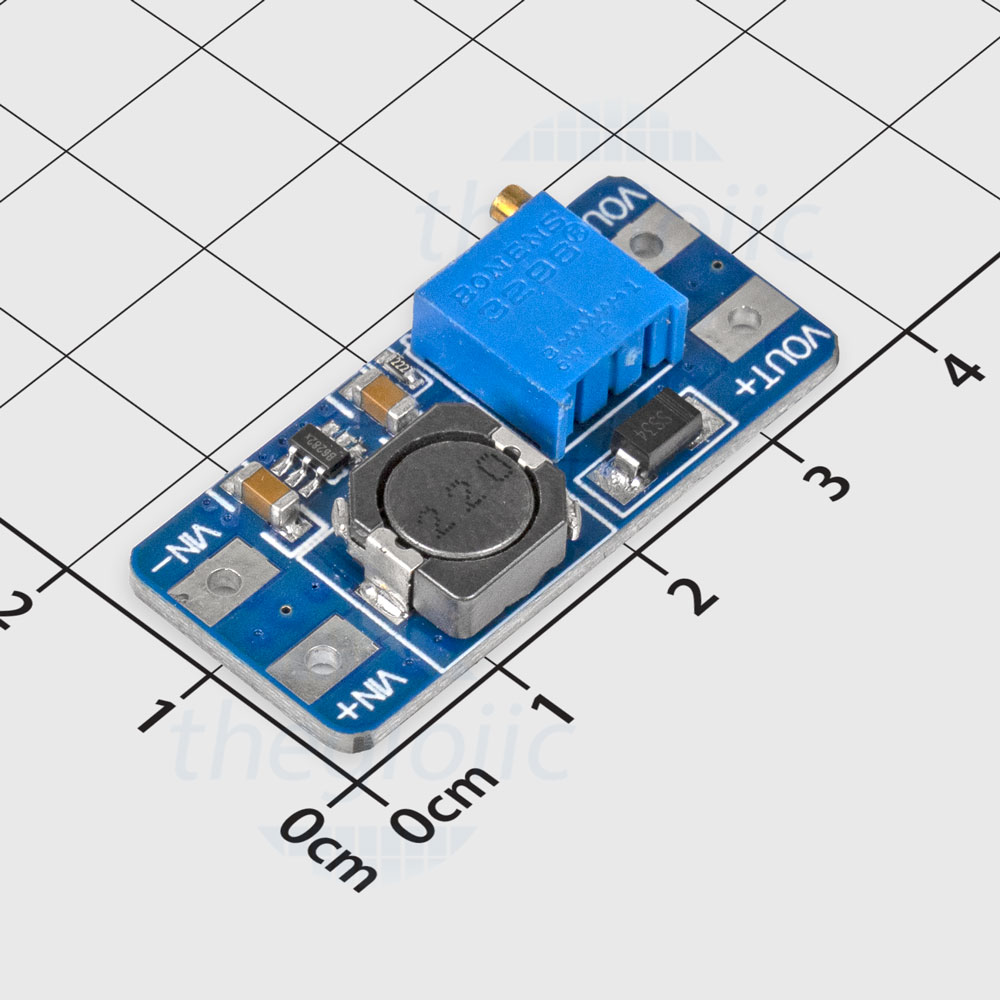
\includegraphics[width = 0.4\textwidth]{img/4.png}
    \caption{Mạch MT3608}
\end{figure}

\noindent\textbf{Thông số kỹ thuật:}
\begin{itemize}
    \item Điện áp đầu vào (VIN): 2V đến 24V.
    \item Điện áp đầu ra (VOUT): Có thể điều chỉnh lên đến tối đa 28V (thông qua biến trở).
    \item Dòng điện đầu ra: Tối đa 2A (dòng đỉnh của switch).
    \item Tần số chuyển mạch: Cố định ở mức 1.2MHz.
    \item Cơ chế điều khiển: Chế độ dòng điện đỉnh (Peak Current Mode Control) giúp ổn định điện áp đầu ra nhanh chóng.
    \item Hiệu suất: Cao (giảm thiểu tổn hao nhiệt).
\end{itemize}
\textbf{Chức năng các chân cơ bản:}
\begin{itemize}
    \item VIN (Chân 5): Chân cấp nguồn đầu vào.
    \item GND (Chân 2): Chân nối đất (Mass).
    \item SW (Chân 1): Chân chuyển mạch, nối với cuộn cảm và cực Anode của Diode. Đây là chân dao động điện áp cao.
    \item FB (Chân 3): Chân hồi tiếp (Feedback). IC so sánh điện áp tại chân này với tham chiếu 0.6V để điều chỉnh điện áp ra $V_{OUT}=0.6V \times \left(1+\dfrac{R_1}{R_2}\right)$
    \item EN (Chân 4): Chân cho phép (Enable). Mức cao (>1.5V) để bật mạch, mức thấp (<0.4V) để tắt mạch (về chế độ chờ tiết kiệm điện).
\end{itemize}
Mạch hoạt động dựa trên nguyên lý tích trữ và giải phóng năng lượng qua cuộn cảm L1:
\begin{enumerate}
    \item Pha tích năng lượng (MOSFET Bật): Dòng điện chạy qua cuộn cảm L1 xuống mass, năng lượng được lưu trữ dưới dạng từ trường. Diode D1 khóa, tụ C2 cấp điện cho tải.
    \item Pha xả năng lượng (MOSFET Tắt): Cuộn cảm đảo cực tính, tạo điện áp cảm ứng cộng hưởng với nguồn vào đẩy qua Diode D1 để nạp cho tụ C2 và cấp cho tải với điện áp cao hơn.
\end{enumerate}